\tikzsetfigurename{module3_fig_LoRa}
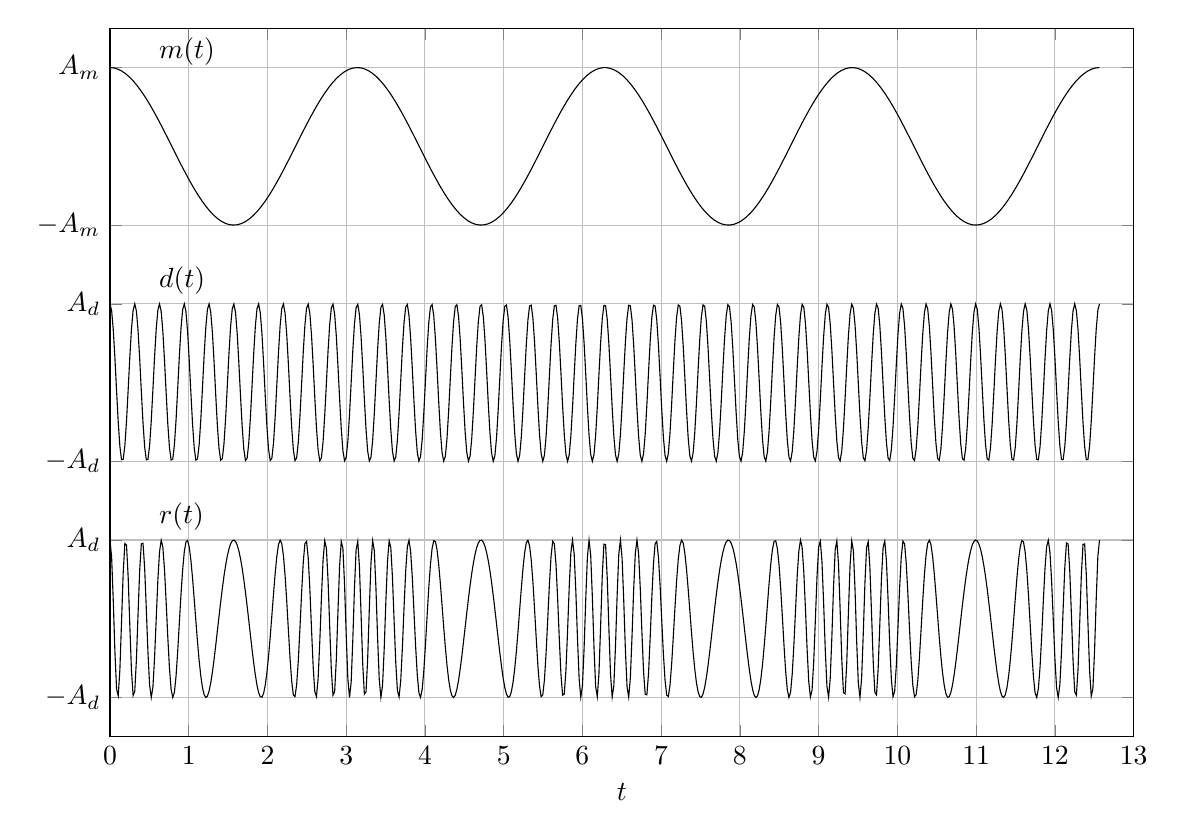
\begin{tikzpicture}
    \begin{axis}[
        grid=both,
        x=1cm,y=1cm,
        ymin = -7.5, ymax=1.5,
        xmin = 0, xmax = 13,
        xlabel = $t$,
        ytick={-1,1,-4,-2,-7,-5},
        yticklabels={$-A_m$, $A_m$,$-A_d$,$A_d$,$-A_d$,$A_d$}
    ]
      \addplot[domain=0:4*pi,black,samples=250] {cos(x*2*180/pi)};
    \addplot[domain=0:4*pi,black,samples=600] {cos(x*20*180/pi)-3};
      \addplot[domain=0:4*pi,black,samples=600] {cos((x*20 + 6*sin(x*2*180/pi))*180/pi)-6};
      
      \node[above,right] at (0.5,1.2) {$m(t)$};
      \node[above,right] at (0.5,-1.7) {$d(t)$};
      \node[above,right] at (0.5,-4.7) {$r(t)$};
    \end{axis}
\end{tikzpicture}